\section{Plugin\-Manager Class Reference}
\label{classPluginManager}\index{PluginManager@{PluginManager}}
{\tt \#include $<$pluginmanager.h$>$}

\subsection*{Static Public Member Functions}
\begin{CompactItemize}
\item 
KTrader::Offer\-List {\bf query} (const QString \&constraint=QString::null)
\item 
{\bf Plugin} $\ast$ {\bf create\-From\-Query} (const QString \&constraint=QString::null)
\item 
{\bf Plugin} $\ast$ {\bf create\-From\-Service} (const KService::Ptr service)
\item 
void {\bf unload} ({\bf Plugin} $\ast$plugin)
\item 
KService::Ptr {\bf get\-Service} (const {\bf Plugin} $\ast$plugin)
\item 
void {\bf dump} (const KService::Ptr service)
\end{CompactItemize}
\subsection*{Static Public Attributes}
\begin{CompactItemize}
\item 
const int {\bf Framework\-Version} = 2
\end{CompactItemize}
\subsection*{Static Private Member Functions}
\begin{CompactItemize}
\item 
vector$<$ {\bf Store\-Item} $>$::iterator {\bf lookup\-Plugin} (const {\bf Plugin} $\ast$plugin)
\end{CompactItemize}
\subsection*{Static Private Attributes}
\begin{CompactItemize}
\item 
vector$<$ {\bf Store\-Item} $>$ {\bf m\_\-store}
\end{CompactItemize}


\subsection{Member Function Documentation}
\index{PluginManager@{Plugin\-Manager}!createFromQuery@{createFromQuery}}
\index{createFromQuery@{createFromQuery}!PluginManager@{Plugin\-Manager}}
\subsubsection{\setlength{\rightskip}{0pt plus 5cm}{\bf Plugin} $\ast$ Plugin\-Manager::create\-From\-Query (const QString \& {\em constraint} = QString::null)\hspace{0.3cm}{\tt  [static]}}\label{classPluginManager_PluginManagere1}


Load and instantiate plugin from query \begin{Desc}
\item[Parameters:]
\begin{description}
\item[{\em constraint}]A constraint to limit the choices returned, QString::null to get all services of the given {\tt servicetype} \end{description}
\end{Desc}
\begin{Desc}
\item[Returns:]Pointer to {\bf Plugin}{\rm (p.\,\pageref{classPlugin})}, or NULL if error \end{Desc}
\begin{Desc}
\item[See also:]{\tt http://developer.kde.org/documentation/library/kdeqt/tradersyntax.html} \end{Desc}


Definition at line 51 of file pluginmanager.cpp.

References create\-From\-Service(), and query().



\footnotesize\begin{verbatim}52 {
53     KTrader::OfferList offers = query( constraint );
54 
55     if ( offers.isEmpty() ) {
56         kdWarning() << k_funcinfo << "No matching plugin found.\n";                                          
57         return 0;
58     }
59                 
60     return createFromService( *offers.begin() );    
61 }
\end{verbatim}\normalsize 


Here is the call graph for this function:\begin{figure}[H]
\begin{center}
\leavevmode
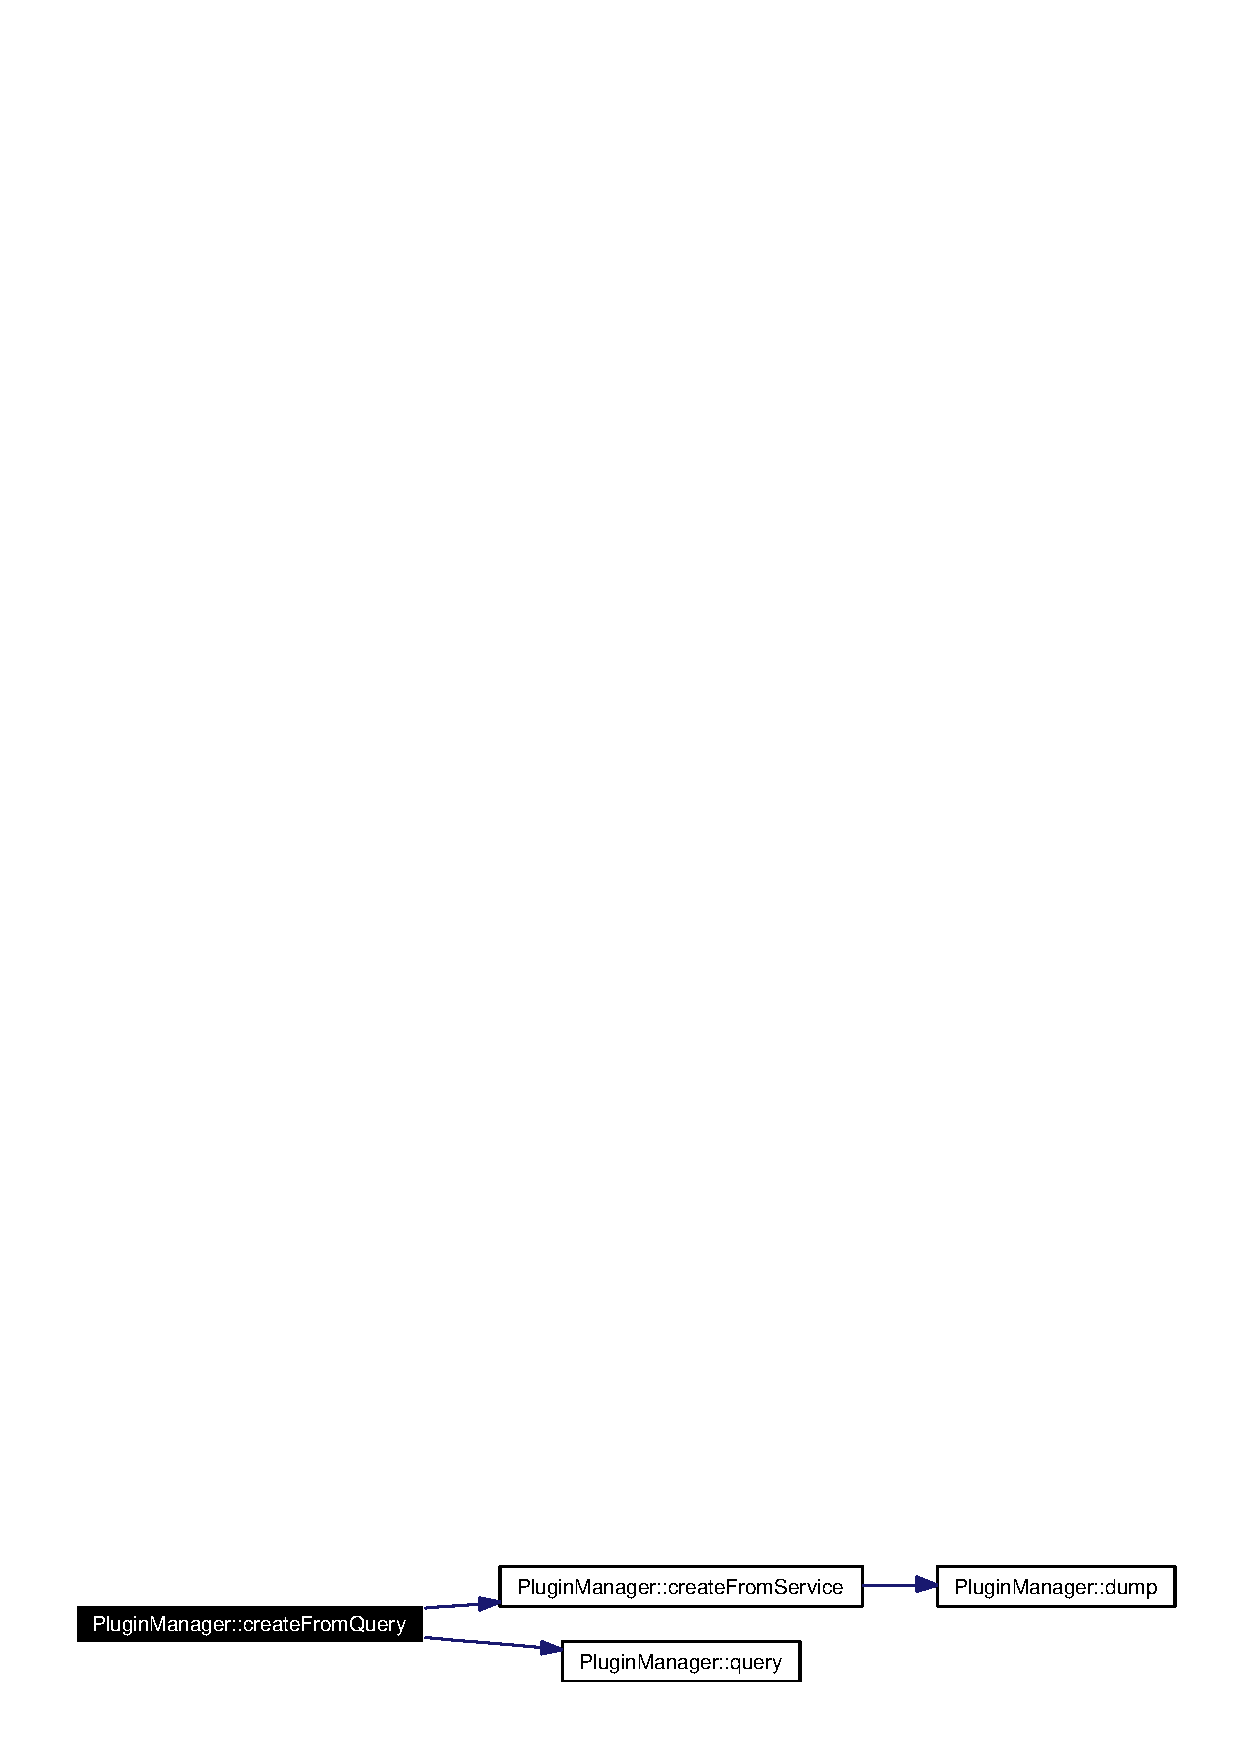
\includegraphics[width=282pt]{classPluginManager_PluginManagere1_cgraph}
\end{center}
\end{figure}
\index{PluginManager@{Plugin\-Manager}!createFromService@{createFromService}}
\index{createFromService@{createFromService}!PluginManager@{Plugin\-Manager}}
\subsubsection{\setlength{\rightskip}{0pt plus 5cm}{\bf Plugin} $\ast$ Plugin\-Manager::create\-From\-Service (const KService::Ptr {\em service})\hspace{0.3cm}{\tt  [static]}}\label{classPluginManager_PluginManagere2}


Load and instantiate plugin from service \begin{Desc}
\item[Parameters:]
\begin{description}
\item[{\em service}]Pointer to KService \end{description}
\end{Desc}
\begin{Desc}
\item[Returns:]Pointer to {\bf Plugin}{\rm (p.\,\pageref{classPlugin})}, or NULL if error \end{Desc}


Definition at line 65 of file pluginmanager.cpp.

References dump(), Plugin\-Manager::Store\-Item::library, m\_\-store, Plugin\-Manager::Store\-Item::plugin, and Plugin\-Manager::Store\-Item::service.

Referenced by create\-From\-Query().



\footnotesize\begin{verbatim}66 {
67     kdDebug() << k_funcinfo << "Trying to load: " << service->library() << endl;
68     
69     //get the library loader instance
70     KLibLoader *loader = KLibLoader::self();
71     //try to load the specified library
72     KLibrary *lib = loader->globalLibrary( QFile::encodeName( service->library() ) );
73 
74     if ( !lib ) {
75         kdWarning() << k_funcinfo << "lib == NULL\n";
76         return 0;
77     }
78     //look up address of init function and cast it to pointer-to-function
79     Plugin* (*create_plugin)() = ( Plugin* (*)() ) lib->symbol( "create_plugin" );
80     
81     if ( !create_plugin ) {
82         kdWarning() << k_funcinfo << "create_plugin == NULL\n";
83         return 0;
84     }
85     //create plugin on the heap
86     Plugin* plugin = create_plugin();
87     
88     //put plugin into store
89     StoreItem item;
90     item.plugin = plugin;
91     item.library = lib;
92     item.service = service;
93     m_store.push_back( item );
94     
95     dump( service );
96     return plugin;
97 }
\end{verbatim}\normalsize 


Here is the call graph for this function:\begin{figure}[H]
\begin{center}
\leavevmode
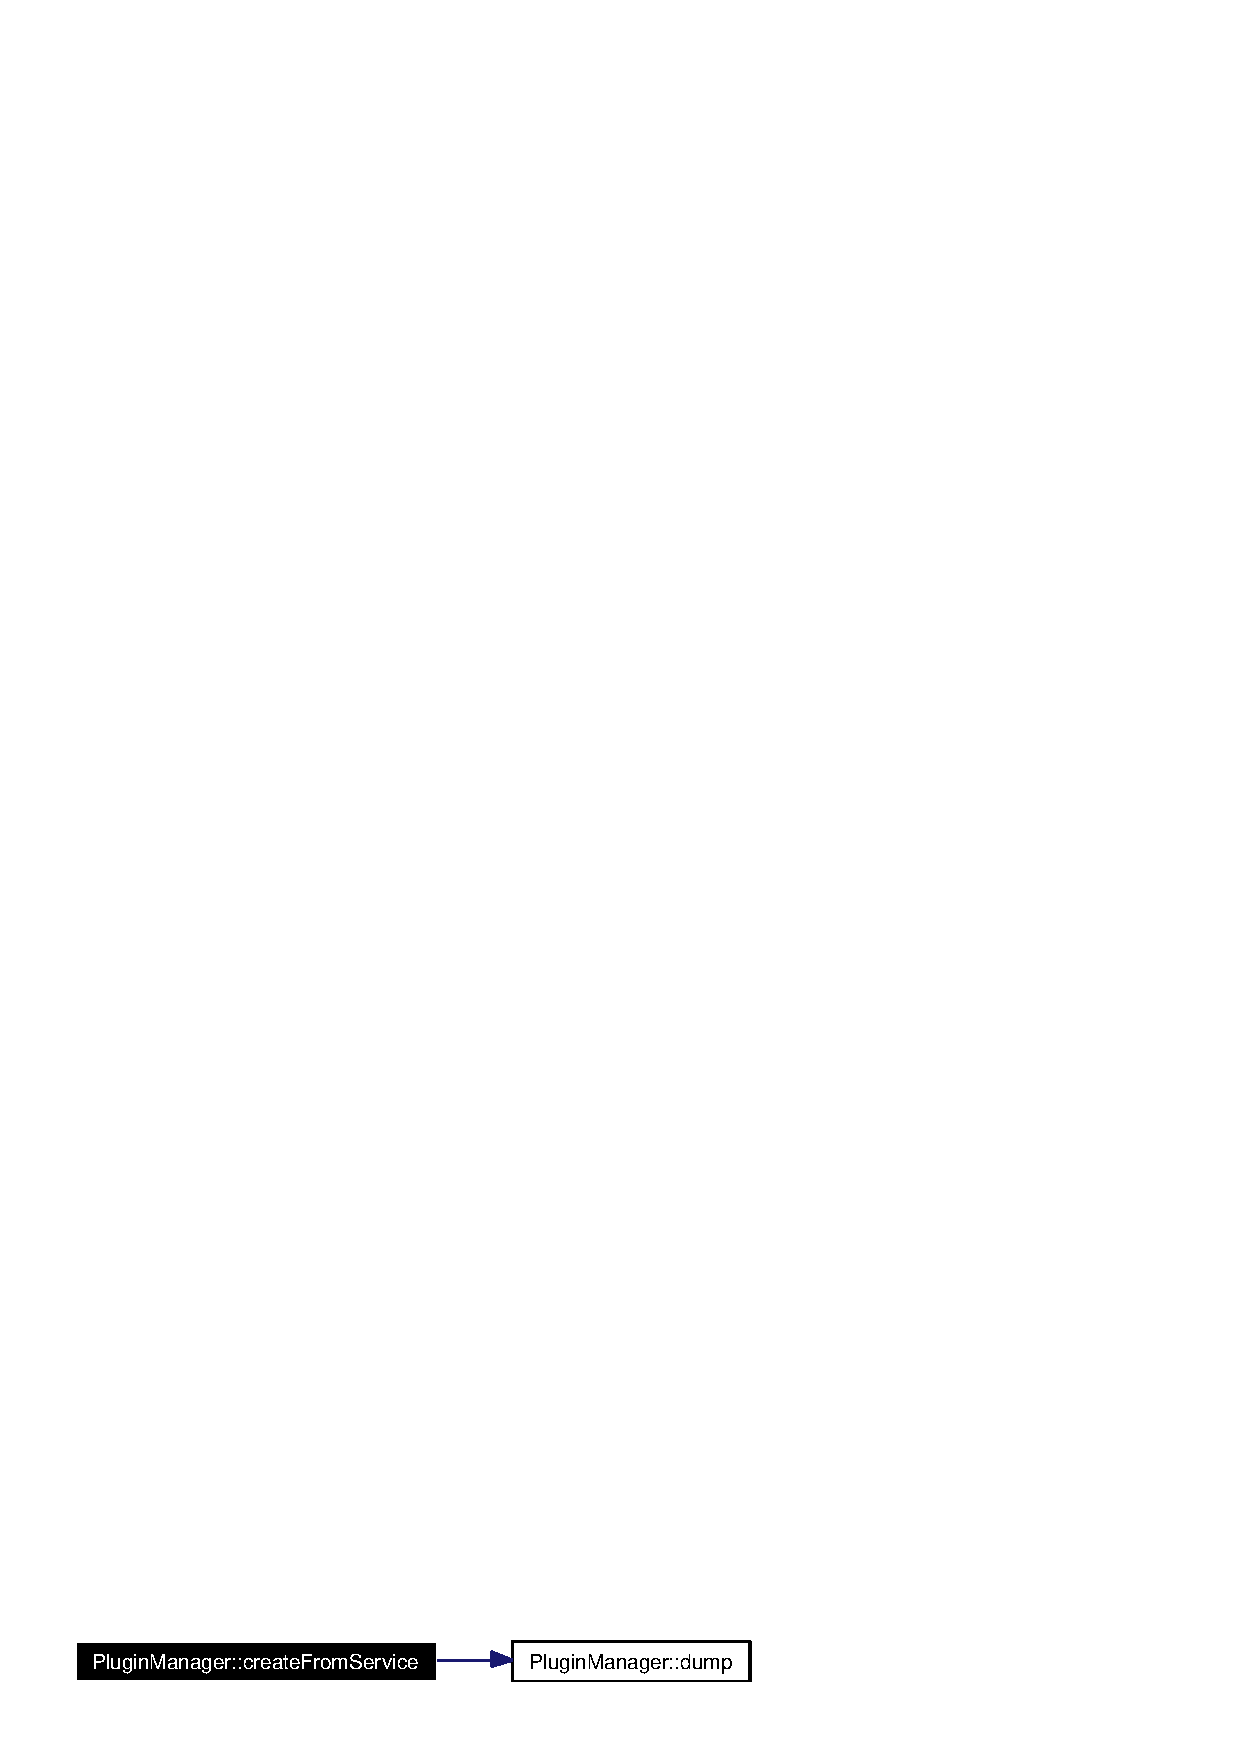
\includegraphics[width=180pt]{classPluginManager_PluginManagere2_cgraph}
\end{center}
\end{figure}
\index{PluginManager@{Plugin\-Manager}!dump@{dump}}
\index{dump@{dump}!PluginManager@{Plugin\-Manager}}
\subsubsection{\setlength{\rightskip}{0pt plus 5cm}void Plugin\-Manager::dump (const KService::Ptr {\em service})\hspace{0.3cm}{\tt  [static]}}\label{classPluginManager_PluginManagere5}


Dump properties from a service to stdout for debugging \begin{Desc}
\item[Parameters:]
\begin{description}
\item[{\em service}]Pointer to KService \end{description}
\end{Desc}


Definition at line 140 of file pluginmanager.cpp.

Referenced by create\-From\-Service().



\footnotesize\begin{verbatim}141 {
142     assert( service.data() );
143     
144     kdDebug() << endl;
145     
146     kdDebug() << "PluginManager Service DUMP:\n";
147     kdDebug() << "---------------------------\n";
148     kdDebug() << "name                          : "
149                 << service->name()                                                  << endl;
150     kdDebug() << "library                       : "
151                 << service->library()                                               << endl;
152     kdDebug() << "desktopEntryPath              : "
153                 << service->desktopEntryPath()                                      << endl;
154     kdDebug() << "X-KDE-plugintype              : "
155                 << service->property( "X-KDE-amaroK-plugintype" ).toString()        << endl;
156     kdDebug() << "X-KDE-amaroK-authors          : "
157                 << service->property( "X-KDE-amaroK-authors" ).toStringList()       << endl;
158     kdDebug() << "X-KDE-amaroK-version          : "
159                 << service->property( "X-KDE-amaroK-version" ).toString()           << endl;
160     kdDebug() << "X-KDE-amaroK-framework-version: "
161                 << service->property( "X-KDE-amaroK-framework-version" ).toString() << endl;
162     
163     kdDebug() << endl;
164 }
\end{verbatim}\normalsize 
\index{PluginManager@{Plugin\-Manager}!getService@{getService}}
\index{getService@{getService}!PluginManager@{Plugin\-Manager}}
\subsubsection{\setlength{\rightskip}{0pt plus 5cm}KService::Ptr Plugin\-Manager::get\-Service (const {\bf Plugin} $\ast$ {\em plugin})\hspace{0.3cm}{\tt  [static]}}\label{classPluginManager_PluginManagere4}


Look up service for loaded plugin from store \begin{Desc}
\item[Parameters:]
\begin{description}
\item[{\em pointer}]Pointer to plugin \end{description}
\end{Desc}
\begin{Desc}
\item[Returns:]KService, or 0 if not found \end{Desc}


Definition at line 120 of file pluginmanager.cpp.

References lookup\-Plugin(), and m\_\-store.



\footnotesize\begin{verbatim}121 {
122     kdDebug() << k_funcinfo << endl;
123     
124     if ( !plugin ) {
125         kdWarning() << k_funcinfo << "pointer == NULL\n";   
126         return 0;
127     }
128        
129     //search plugin in store
130     vector<StoreItem>::const_iterator iter = lookupPlugin( plugin ); 
131     
132     if ( iter == m_store.end() ) 
133         kdWarning() << k_funcinfo << "Plugin not found in store.\n";
134     
135     return (*iter).service;
136 }
\end{verbatim}\normalsize 


Here is the call graph for this function:\begin{figure}[H]
\begin{center}
\leavevmode
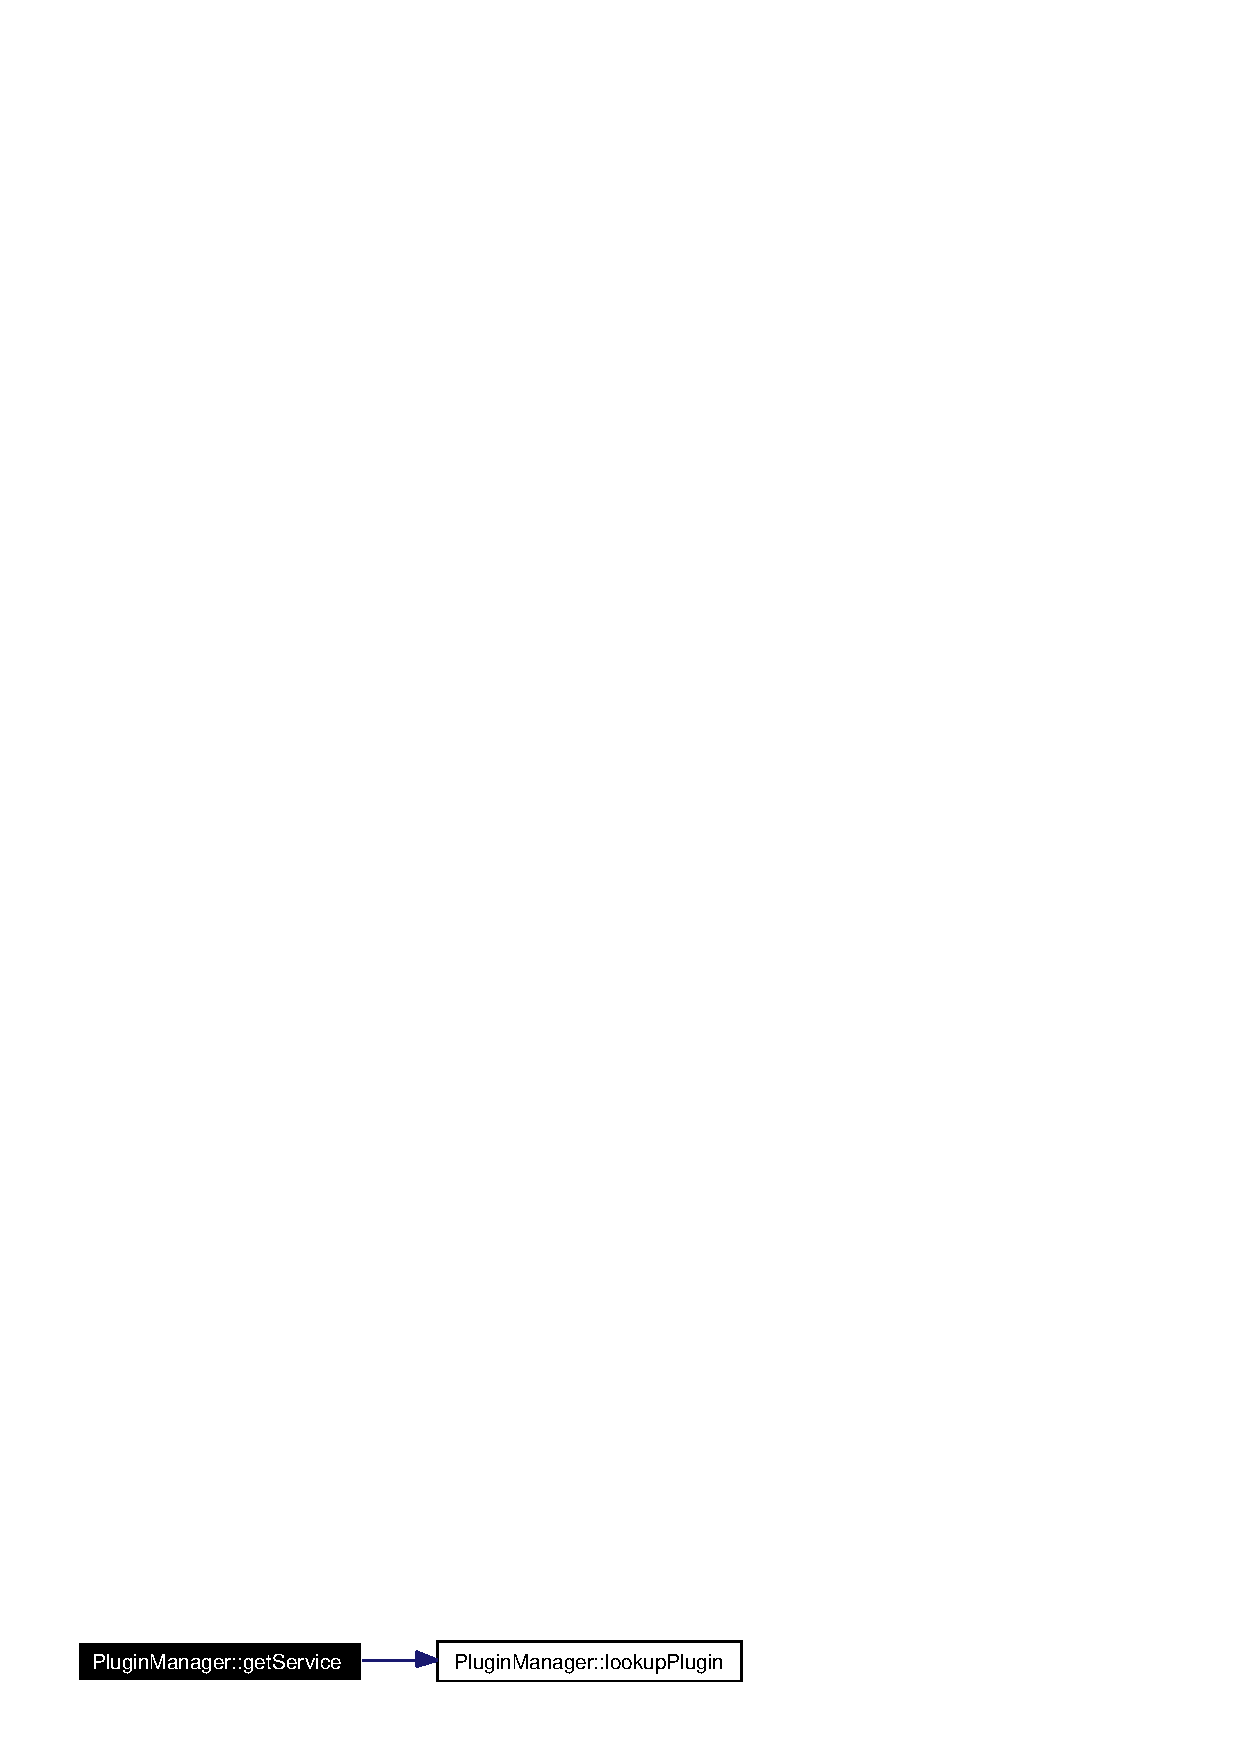
\includegraphics[width=178pt]{classPluginManager_PluginManagere4_cgraph}
\end{center}
\end{figure}
\index{PluginManager@{Plugin\-Manager}!lookupPlugin@{lookupPlugin}}
\index{lookupPlugin@{lookupPlugin}!PluginManager@{Plugin\-Manager}}
\subsubsection{\setlength{\rightskip}{0pt plus 5cm}vector$<$ {\bf Plugin\-Manager::Store\-Item} $>$::iterator Plugin\-Manager::lookup\-Plugin (const {\bf Plugin} $\ast$ {\em plugin})\hspace{0.3cm}{\tt  [static, private]}}\label{classPluginManager_PluginManagerh0}




Definition at line 172 of file pluginmanager.cpp.

References m\_\-store.

Referenced by get\-Service(), and unload().



\footnotesize\begin{verbatim}173 {
174     vector<StoreItem>::iterator iter; 
175     
176     //search plugin pointer in store
177     for ( iter = m_store.begin(); iter != m_store.end(); iter++ ) {
178         if ( (*iter).plugin == plugin )
179             break;
180     }
181 
182     return iter;
183 }
\end{verbatim}\normalsize 
\index{PluginManager@{Plugin\-Manager}!query@{query}}
\index{query@{query}!PluginManager@{Plugin\-Manager}}
\subsubsection{\setlength{\rightskip}{0pt plus 5cm}KTrader::Offer\-List Plugin\-Manager::query (const QString \& {\em constraint} = QString::null)\hspace{0.3cm}{\tt  [static]}}\label{classPluginManager_PluginManagere0}


It will return a list of services that match your specifications. The only required parameter is the service type. This is something like 'text/plain' or 'text/html'. The constraint parameter is used to limit the possible choices returned based on the constraints you give it.

The {\tt constraint} language is rather full. The most common keywords are AND, OR, NOT, IN, and EXIST, all used in an almost spoken-word form. An example is: 

\footnotesize\begin{verbatim} (Type == 'Service') and (('KParts/ReadOnlyPart' in ServiceTypes) or (exist Exec))
\end{verbatim}
\normalsize


The keys used in the query (Type, Service\-Type, Exec) are all fields found in the .desktop files.

\begin{Desc}
\item[Parameters:]
\begin{description}
\item[{\em constraint}]A constraint to limit the choices returned, QString::null to get all services of the given {\tt servicetype} \end{description}
\end{Desc}
\begin{Desc}
\item[Returns:]A list of services that satisfy the query \end{Desc}
\begin{Desc}
\item[See also:]{\tt http://developer.kde.org/documentation/library/kdeqt/tradersyntax.html} \end{Desc}


Definition at line 37 of file pluginmanager.cpp.

References Framework\-Version.

Referenced by create\-From\-Query().



\footnotesize\begin{verbatim}38 {    
39     // Add versioning constraint
40     QString str = QString( "[X-KDE-amaroK-framework-version] >= %1 and " )
41                      .arg( FrameworkVersion );
42     
43     kdDebug() << k_funcinfo << endl
44               << "Plugin trader constraint: " << str + constraint << endl;
45     
46     return KTrader::self()->query( "amaroK/Plugin", str + constraint );
47 }    
\end{verbatim}\normalsize 
\index{PluginManager@{Plugin\-Manager}!unload@{unload}}
\index{unload@{unload}!PluginManager@{Plugin\-Manager}}
\subsubsection{\setlength{\rightskip}{0pt plus 5cm}void Plugin\-Manager::unload ({\bf Plugin} $\ast$ {\em plugin})\hspace{0.3cm}{\tt  [static]}}\label{classPluginManager_PluginManagere3}


Remove library and delete plugin \begin{Desc}
\item[Parameters:]
\begin{description}
\item[{\em plugin}]Pointer to plugin \end{description}
\end{Desc}


Definition at line 101 of file pluginmanager.cpp.

References lookup\-Plugin(), and m\_\-store.



\footnotesize\begin{verbatim}102 {
103     kdDebug() << k_funcinfo << endl;
104     
105     vector<StoreItem>::iterator iter = lookupPlugin( plugin ); 
106             
107     if ( iter != m_store.end() ) {
108         delete (*iter).plugin;
109         kdDebug() << "Unloading library: "<< (*iter).service->library() << endl;
110         (*iter).library->unload();
111         
112         m_store.erase( iter );
113     }
114     else
115         kdWarning() << k_funcinfo << "Could not unload plugin (not found in store).\n";
116 }
\end{verbatim}\normalsize 


Here is the call graph for this function:\begin{figure}[H]
\begin{center}
\leavevmode

\includegraphics[width=169pt]{classPluginManager_PluginManagere3_cgraph}
\end{center}
\end{figure}


\subsection{Member Data Documentation}
\index{PluginManager@{Plugin\-Manager}!FrameworkVersion@{FrameworkVersion}}
\index{FrameworkVersion@{FrameworkVersion}!PluginManager@{Plugin\-Manager}}
\subsubsection{\setlength{\rightskip}{0pt plus 5cm}const int {\bf Plugin\-Manager::Framework\-Version} = 2\hspace{0.3cm}{\tt  [static]}}\label{classPluginManager_PluginManagers0}


Bump this number whenever the plugin framework gets incompatible with older versions 

Definition at line 32 of file pluginmanager.h.

Referenced by query().\index{PluginManager@{Plugin\-Manager}!m_store@{m\_\-store}}
\index{m_store@{m\_\-store}!PluginManager@{Plugin\-Manager}}
\subsubsection{\setlength{\rightskip}{0pt plus 5cm}vector$<$ {\bf Plugin\-Manager::Store\-Item} $>$ {\bf Plugin\-Manager::m\_\-store}\hspace{0.3cm}{\tt  [static, private]}}\label{classPluginManager_PluginManagerv0}




Definition at line 29 of file pluginmanager.cpp.

Referenced by create\-From\-Service(), get\-Service(), lookup\-Plugin(), and unload().

The documentation for this class was generated from the following files:\begin{CompactItemize}
\item 
{\bf pluginmanager.h}\item 
{\bf pluginmanager.cpp}\end{CompactItemize}
